\subsubsection{Podnošenje prijave}
\label{subsubsec:prijava}
\begin{itemize}
  \item \textbf{Kratak opis}: Da bi kandidat započeo obuku u auto školi, prvo mora da podnese prijavu za upis. Popunjava online formular, gde unosi svoje lične podatke, koji se nakon potvrde šalju administrativnom radniku. Radnik formira dokumentaciju za kandidata i prosleđuje ih administratoru sistema, koji unosi informacije o kandidatu u sistem.
  \item \textbf{Učesnici}: 
    \begin{itemize} 
      \item Kandidat
      \item Administrativni radnik
      \item Administrator sistema
    \end{itemize} 
  \item \textbf{Preduslovi}:
    \begin{itemize}
    \item Kandidat mora posedovati važeću ličnu kartu.
    \item Kandidat mora uplatiti prvu ratu.
    \end{itemize}
  \item \textbf{Postuslovi}:
      \begin{itemize}
      \item Kandidat ispunjava uslove za prijavu.
      \end{itemize}
  \item \textbf{Osnovni tok}:
      \begin{enumerate}
        \item Kandidat otvara online formu za prijavu u auto školu.
        \item Sistem prikazuje formu kandidatu.
        \item Kandidat popunjava formu, unoseći sve potrebne informacije.
        \item Kanidat šalje unete podatke klikom na dugme “Pošalji”.
        \item Sistem validira unos podataka.
        \item Sistem čuva podatke.
        \item Sistem prosleđuje podatke administrativnom radniku.
        \item Аdministrativni radnik proverava da li kanidat ispunjava uslove za upis.
        \item Administrativni radnik formira dokumentaciju za kandidata.
        \item Administrativni radnik prosleđuje podatke o kandidatu administratoru sistema.
      \end{enumerate}

  \item \textbf{Alternativni tokovi}:
      \begin{itemize}
        \item A1. \textbf{Kandidat nije uneo ispravne podatke.}
        Ukoliko je u koraku 5 sistem uočio nevalidnost u formatu unetih podataka od strane kandidata, neophodno je da ih kandidat unese ponovo u ispravnom obliku.
        Proces se nastavlja u koraku 1 osnovnog toka.
        \item A2. \textbf{Kandidat ne ispunjava uslove za upis.}
        Ukoliko je u koraku 8 administrativni radnik uočio da kandidat ne ispunjava uslove za prijavu, kontaktira ga kako bi ga obavestio o tome.
        Kandidat se ne može upisati u auto školu i proces se završava.
      \end{itemize}

  \item \textbf{Dodatne informacije}:\newline
  Potrebni podaci za prijavu su ime, prezime, JMBG, broj telefona, imejl adresa i potvrda o uplati prve rate.
\end{itemize}

\begin{figure}[H]
  \begin{center}
      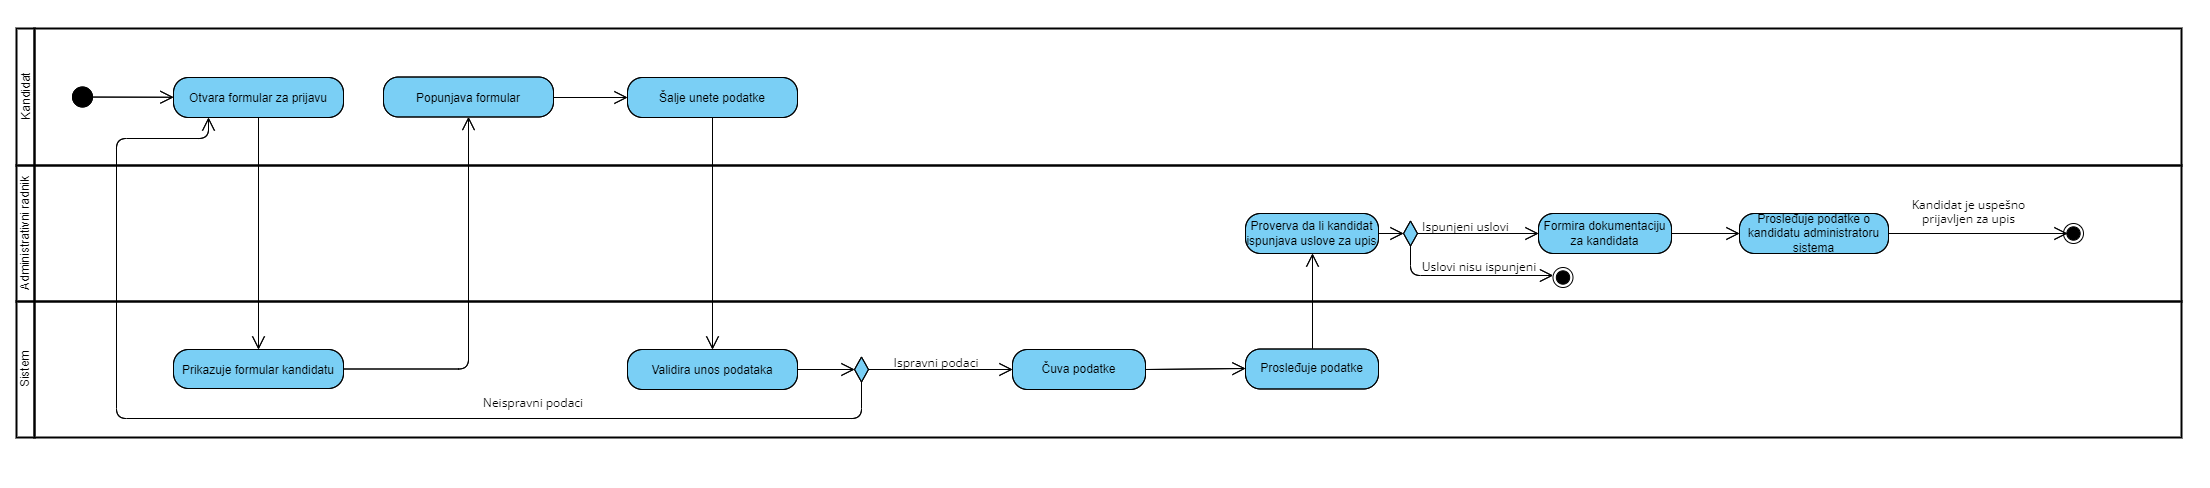
\includegraphics[width=140mm, height=70mm]{Diagrams/dijagram_aktivnosti_podnosenje_prijave.png}
  \end{center}
  \caption {Dijagram aktivnosti - Podnošenje prijave}
  \label{activity_podnosenje_prijave}

\end{figure}



